\section{Proposed Sliceformer}\label{sec:model}
\subsection{Motivations}
Typically, given an input $\bm{X}\in\mathbb{R}^{N\times d}$, where $N$ indicates the length of a sequence or the size of a sample set and $d$ is the input feature dimension, an attention head first obtains the value, query, and key matrices by linear maps, i.e., $\bm{V}=\bm{X}\bm{W}_V\in\mathbb{R}^{N\times D}$, $\bm{Q}=\bm{X}\bm{W}_Q\in\mathbb{R}^{N\times D}$, and $\bm{K}=\bm{X}\bm{W}_K\in\mathbb{R}^{N\times D}$, and then projects $\bm{V}$ as follows:
\begin{eqnarray}\label{eq:att}
\begin{aligned}
    \text{Attention}(\bm{V};\bm{Q},\bm{K}):=\bm{P}(\bm{Q},\bm{K})\bm{V}. 
\end{aligned}
\end{eqnarray}
Here, we take $\bm{V}$ as the input of the head, and $\bm{P}(\bm{Q},\bm{K})\in\mathbb{R}^{N\times N}$ is the attention map parametrized by $\bm{Q}$ and $\bm{K}$. 
The multi-head attention layer applies a group of linear maps, i.e., $\theta=\{\bm{W}_{V,m},\bm{W}_{Q,m},\bm{W}_{K,m}\in\mathbb{R}^{d\times D}\}_{m=1}^{M}$, to construct $M$ attention heads and concatenates their outputs, i.e.,
\begin{eqnarray}\label{eq:mha}
\begin{aligned}
    &\text{MHA}_{\theta}(\bm{X}) := \text{Concat}_{\text{row}}(\{\text{Attention}(\bm{V}_m;\bm{Q}_m,\bm{K}_m)\}_{m=1}^{M})\in\mathbb{R}^{N\times MD},\\
    &\text{where}~\bm{V}_m=\bm{X}\bm{W}_{V,m},~\bm{Q}_m=\bm{X}\bm{W}_{Q,m},~\text{and}~\bm{K}_m=\bm{X}\bm{W}_{K,m},~\forall m=1,...,M.
\end{aligned}
\end{eqnarray}
In this study, we aim to propose a surrogate of the MHA mechanism in~\eqref{eq:mha}. 
The design of our model is motivated by the following observations and analysis. 

\begin{figure}[t]
    \centering
    \begin{minipage}[t]{0.4\linewidth}
    \begin{algorithm}[H]
    \small{
    	\caption{Numerical Test of Softmax}\label{alg:softmax}
    	\begin{algorithmic}[1]
    	\STATE \texttt{x = torch.randn(N)}
        \STATE \texttt{index = torch.randperm(N)}
        \STATE \texttt{y1 = torch.softmax(x)[index]}
        \STATE \texttt{y2 = torch.softmax(x[index])} 
        \STATE \texttt{Std = torch.std(y1)}
        \STATE \texttt{MAE = torch.norm(y1-y2, p=1)}
        \STATE \texttt{Prob = torch.sum(y1==y2) / N}
    	\end{algorithmic}
    }
    \end{algorithm}
    \end{minipage}
    \begin{minipage}[t]{0.58\linewidth}
    \subfigure[]{
    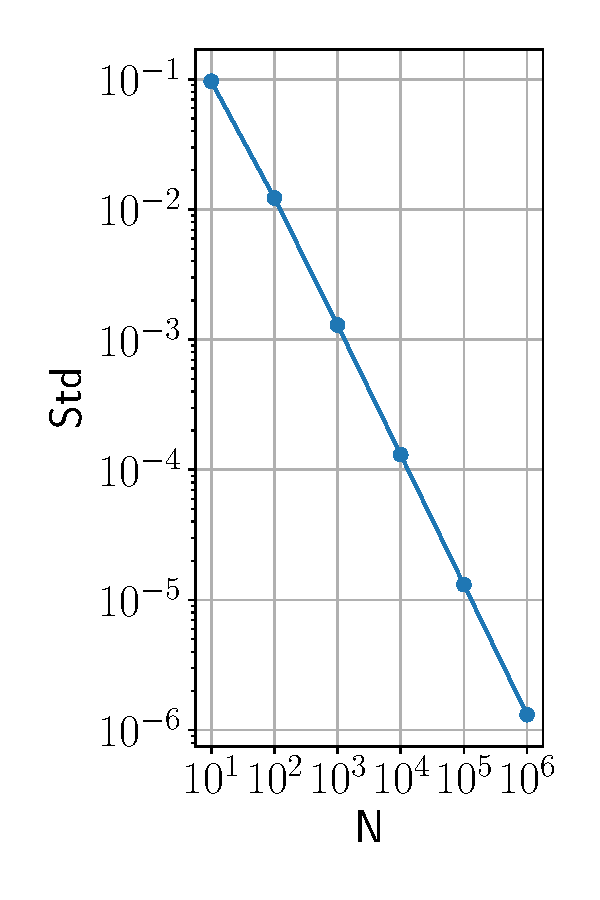
\includegraphics[height=3.8cm]{figures/softmax_std.pdf}\label{fig:sm-std}
    }
    \subfigure[]{
    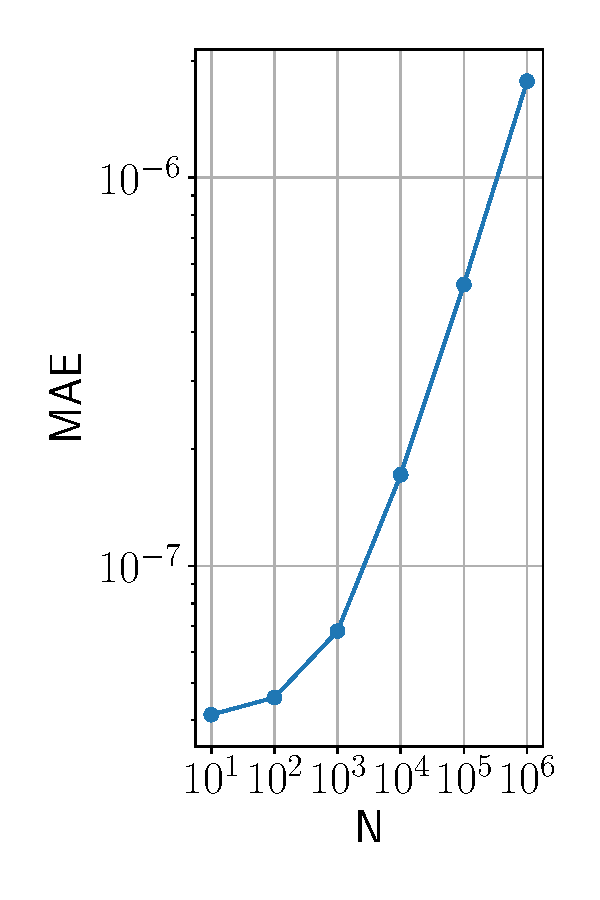
\includegraphics[height=3.8cm]{figures/softmax_err.pdf}\label{fig:sm-err}
    }
    \subfigure[]{
    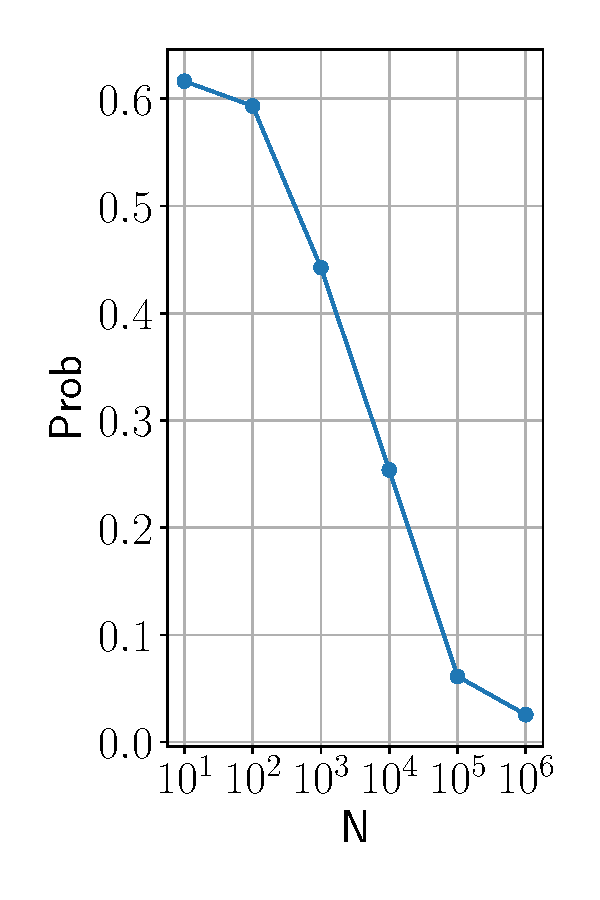
\includegraphics[height=3.8cm]{figures/softmax_count.pdf}\label{fig:sm-count}
    }
    \end{minipage}
    \caption{Algorithm~\ref{alg:softmax} shows the PyTorch code used to verify the numerical issues of the softmax operation. 
    Setting the sequence length $N\in\{10,...,10^6\}$, we run the code $100$ trials with Pytorch 2.0.0 and Python 3.9. 
    With the increase of $N$, (a) the softmax operation suffers from the over-smoothness issue, and (b, c) the exchange of the softmax operation and the permutation operation destructs the permutation-equivariance of output numerically.}
    \label{fig:softmax}
\end{figure}


\textbf{Numerical Issues of Softmax.} 
Table~\ref{tab:cmp} shows that most existing attention maps are implemented based on the softmax operation. 
The softmax operation makes the attention maps dense and row-stochastic, which suffers from numerical issues when dealing with long sequences. 
Firstly, it has been well-known that the output of the softmax operation tends to be over-smoothed with the increase of data size --- the standard deviation of the output elements reduces rapidly, as shown in Figure~\ref{fig:sm-std}.
Without any additional data preprocessing like LSH~\cite{kitaev2020reformer} or sliding windows~\cite{beltagy2020longformer,child2019generating}, the softmax operation always leads to over-smoothed attention maps for long sequences. 

Secondly, we observe a numerical issue seldom considered by existing work, called the ``destruction of permutation-equivariance (DPE)''. 
In particular, the softmax operation should be permutation-equivariant in theory, i.e., $\text{Softmax}_{\sigma}(\bm{x})=\text{Softmax}(\bm{x}_{\sigma})$ for an arbitrary vector $\bm{x}$ and its index permutation $\sigma$. 
To our surprise, however, this property cannot be held in practice --- the exchange of the softmax operation and the permutation operation leads to different outputs, as shown in Figures~\ref{fig:sm-err} and~\ref{fig:sm-count}. 
With the increase in data size, the mean absolute error between the outputs increases, and the probability of appearing identical elements decreases. 
Stacking multiple softmax-based attention layers may make the DPE issue more severe.
Suppressing the DPE problem is necessary for the Transformers modeling structured data as sequences (e.g., the ViT~\cite{dosovitskiy2021an} modeling images as sequences of patches) because the attention maps destructing the permutation-equivariance property may result in permutation-variant data representations.

\textbf{Recent Advances in Attention Models.}
As Figure~\ref{fig:cmp}, the following experiments, and the results in~\cite{beltagy2020longformer,gu2021efficiently,zhen2022cosformer,ma2022mega} show, the models applying sparse attention maps, e.g., CosFormer~\cite{zhen2022cosformer} and Longformer~\cite{beltagy2020longformer}, can achieve competitive performance and higher efficiency than the vanilla Transformer. 
On the contrary, although imposing low-rank structures on the attention maps can also reduce the computational complexity, it seems to harm the performance --- the gaps between the vanilla Transformer and the models using low-rank attention maps (e.g., Local Attention~\cite{tay2021long} and Linear Trans.~\cite{katharopoulos2020transformers}) are significant on the LRA benchmark. 
In our opinion, a potential reason for this phenomenon is that when $\text{rank}(\bm{P})\ll N$, the rank of the output embeddings $\text{MHA}_{\theta}(\bm{X})$ is likely to be smaller than $N$. 
The low-rank structure may limit the representation power of the output embeddings. 
In addition, the recent work in~\cite{sander2022sinkformers} shows that in various discriminative learning tasks, the attention maps tend to be doubly stochastic (i.e., $\bm{P}\bm{1}_N=\bm{1}_N$ and $\bm{P}^{\top}\bm{1}_N=\bm{1}_N$) during training.\footnote{See Figure 2 in~\cite{sander2022sinkformers} for more details.} 
Accordingly, the Sinkformer designs the attention maps based on the Sinkhorn-Knopp algorithm~\cite{sinkhorn1967concerning} and makes them doubly stochastic strictly, achieving better performance than the vanilla Transformer. 

\textbf{Restricted Capacity of Multi-Head Architecture.}
In our opinion, the multi-head architecture is designed to balance model capacity and computational complexity. 
The MHA projects the input to different latent spaces and applies one attention map to each value matrix~\cite{vaswani2017attention}, as shown in~\eqref{eq:mha}. 
The features within a value matrix, i.e., the columns of $\bm{V}$, share the same attention map $\bm{P}$, so we only need to compute one attention map for $D$ features. 
Although such an architecture has better capacity than the single-head attention layer, it does not maximize the capacity of the attention layer.  
In particular, given $MD$ features $\{\bm{V}_m\in\mathbb{R}^{N\times D}\}_{m=1}^{M}$, computing a specialized attention map for each feature can maximize the model capacity but leads to high computational complexity.
Therefore, the solution of the multi-head attention layer is to group the features by $M$ heads and let the features in the same head share the same attention map. 
In other words, the multi-head attention sacrifices some model capacity for computational efficiency.



\subsection{Design Principle and Implementations}
Based on the above observations and analysis, we propose the following two hypotheses to guide the design of our model. 
\begin{hypothesis}\label{hypo:1}
A desired attention map $\bm{P}$ should be full-rank, sparse, and doubly stochastic.
\end{hypothesis}
\begin{hypothesis}\label{hypo:2}
The multi-head architecture aims to achieve a trade-off between model capacity and computational complexity. 
It might be unnecessary if we can find a surrogate that simultaneously has high capacity and low complexity.
\end{hypothesis}
Hypothesis~\ref{hypo:1} is about the desired structure of the attention map. 
It implies that $i$) the usage of the softmax operation should be avoided, and $ii)$ the parameterization based on the query and key matrices might be unnecessary as long as the attention map can keep the desired structure and be updated during training. 
Hypothesis~\ref{hypo:2} is about the necessity of the multi-head architecture. 
It implies that if we can compute a specialized attention map for each feature with low computational cost, such an operation might be comparable, even superior, to the current MHA mechanism.


We design our Sliceformer based on these two hypotheses. 
As shown in Table~\ref{tab:cmp}, the key contribution of our Sliceformer is implementing a new attention layer based on an extremely simple \textbf{slice-sorting} operation, which projects the input linearly to a latent space and sorts each feature, i.e.,
\begin{eqnarray}\label{eq:ss}
\begin{aligned}
    \text{SliceSort}(\bm{X}) := \text{Sort}_{\text{col}}(\underbrace{\bm{X}\bm{W}_V}_{\bm{V}=[\bm{v}_i]}) = \text{Concat}_{\text{row}}(\{\bm{P}_i\bm{v}_i\}_{i=1}^{MD}) \in\mathbb{R}^{N\times MD},
\end{aligned}
\end{eqnarray}
where $\bm{W}_V\in\mathbb{R}^{d\times MD}$ is the projection matrix,\footnote{Here, we set the number of columns in $\bm{W}_V$ to be $MD$, such that the output has the same shape with the output of MHA.} and $\bm{V}=\bm{XW}_V$. 
Here, we call each column of $\bm{V}$ a ``slice'', denoted as $\bm{v}_i$ for $i=1,...,MD$. 
Each slice corresponds to the projection result of $N$ $d$-dimensional samples in a 1D space. 
As shown in~\eqref{eq:ss}, sorting a slice $\bm{v}_i$ corresponds to the multiplication between a permutation matrix $\bm{P}_i$ and the slice, and accordingly, our slicing-sorting operation concatenates all sorted slices as the output. 

Our slicing-sorting attention layer has some potential advantages compared to the MHA mechanism. 

\textbf{Structured and Efficient Attention Map.}
As shown in~\eqref{eq:ss}, our slicing-sorting operation implements a permutation matrix as an attention map for each feature dimension.
The permutation matrix naturally has the full-rank, sparse, and doubly stochastic structure proposed in Hypothesis~\ref{hypo:1}, leading to a competitive alternative to traditional attention maps.
Moreover, instead of generating an explicit attention map with size $\mathcal{O}(N^2)$, we implement permutation matrix implicitly via sorting, whose space complexity is $\mathcal{O}(\log N)$ in general and $\mathcal{O}(N)$ in the worst case. 

\textbf{Low Complexity and High Capacity.}
Our slicing-sorting operation has high model capacity because it generates a specific attention map for each feature dimension rather than a feature group. 
Given $\bm{V}\in\mathbb{R}^{N\times MD}$, we sort the $MD$ columns, whose computational complexity is $\mathcal{O}(MDN\log N)$. 
On the contrary, the other attention layers merely generate $M$ attention maps, and their computational complexity (i.e., the complexity per head in Table~\ref{tab:cmp} times the number of heads) is at most comparable to ours. 
According to Hypothesis~\ref{hypo:2}, our slicing-sorting attention layer has the potential to outperform the multi-head architecture. 


\textbf{Permutation-Invariance.}
The formulations in Table~\ref{tab:cmp} indicate that traditional attention layers are permutation-equivariant in theory. 
Given the outputs of such layers, we can obtain permutation-invariant data representations by $i)$ pooling the outputs and $ii)$ extracting the outputs of predefined super nodes~\cite{ying2021transformers} or ``CLS'' positions~\cite{vaswani2017attention,dosovitskiy2021an}.
As aforementioned, the permutation-equivariance cannot be held numerically for long sequences because of the DPE problem of the softmax operation. 
As a result, the permutation-invariance of the representation may also suffer from numerical errors. 
On the contrary, the output of our slicing-sorting attention layer is naturally permutation-invariant because $\text{Sort}_{\text{col}}(\bm{V})=\text{Sort}_{\text{col}}(\bm{V}_{\sigma})$ for an arbitrary row index permutation $\sigma$.
The simplicity of our operation ensures that this permutation-invariance can be held without numerical errors. 


\subsection{Variants of Sliceformer}\label{ssec:variants}
Replacing the MHA of the Transformer with our slicing-sorting attention layer leads to our Sliceformer. 
Note that, besides sorting, we can obtain attention matrices by many other methods. 
Here, we provide the following two methods, leading to two variants of Sliceformer. 
\begin{enumerate}
    \item \textbf{Multi-permutation:} 
    Given the permutation matrix $\bm{P}$ derived by sorting, we can derive more permutation matrices by $\bm{P}^{k}$, $k\in\mathbb{Z}_{+}$. 
    Accordingly, for each feature $\bm{v}_i$, we can treat $\sum_{k=1}^{K}\alpha_k\bm{P}_{i}^{k}$ as its attention map, where $\bm{\alpha}=[\alpha_k]$ is in the $(K-1)$-Simplex. 
    We can learn $\bm{\alpha}$ or set it in advance.
    The attention map $\sum_{k=1}^{K}\alpha_k\bm{P}_{i}^{k}\bm{v}_i$ can be implemented implicitly by sorting $\bm{v}_i$ once, permuting its elements $K$ times based on the same index order, and averaging the results.
    Its computational complexity is comparable to the sorting operation.
    \item \textbf{Max-exchange:} 
    For each feature $\bm{v}_i$, we find its maximum element and exchange it with the first element, whose computational complexity is $\mathcal{O}(N)$ in time and $\mathcal{O}(1)$ in space. 
\end{enumerate}
In the following experiments, the variants of our Sliceformer help to provide insights into the performance of our Sliceformer and the rationality of the proposed hypotheses.